\chapter{Attacco all'autenticazione delle reti 2G-4G}
Le reti cellulari dal 2G al 4G condividono lo stesso schema architetturale, per questo gran parte delle vulnerabilità che vengono
utilizzate negli attacchi di tipo \textit{denial of service} sono comuni.
Ci sono numerosi modi per effettuare un attacco DOS all'autenticazione già accennati nella sezione 4.1.4, in questo capitolo verranno messe in pratica 
nelle reti 2G fino al 4G.\\
Fondamentalmente, in modo da creare un \textit{denial of service} nel \textit{core network} di una rete cellulare tramite una richiesta di autenticazione bisogna forzare
la computazione dei vettori di autenticazione in modo tale da fare spendere risorse computazionali all'infrastruttura cellulare.
Nel momento che un dispositivo si collega alla rete cellulare si possono verificare le seguenti casistiche:
\begin{itemize}
    \item Se il dispositivo ha una SIM valida inizio la procedura di autenticazione.
    \item Se il dispositivo non ha una SIM valida inizio la procedura di autenticazione ma senza consumare abbastanza risorse nel \textit{network}.
    \item Se il dispositivo non ha una SIM la procedura di autenticazione non viene iniziata.
\end{itemize}
Quindi, è chiaro che per effettuare un DOS al sistema di autenticazione degli utenti è necessario disporre o simulare dei dispositivi con delle SIM valide. La validità della SIM è 
in primo luogo controllata dalla presenza di un IMSI valido come spiegato nella sezione precedente.
Di seguito verranno trattate le principali metodologie per effettuare un DOS al sistema di autenticazione.

\section{Botnet}
Il metodo più conosciuto per creare un \textit{denial of service} a una rete cellulare è tramite una \textit{botnet}.
In questo modo, l'attaccante ha a disposizione un elevato numero di dispositivi con SIM valida che hanno la possibilità di effettuare massivamente una procedura
di autenticazione causando delle dispendiose computazioni all'interno del \textit{network}.\\
In \cite{measuring-dos} è descritto come effettuare un DDOS a una rete cellulare di tipo 2G/3G in modo da esasperare di richieste il suo componente più critico: l'HLR.
Con 11750 dispositivi infettati è possibile degradare le performance della HLR del 93\%\cite{measuring-dos}, garantendo quindi un quasi totale malfunzionamento dell'infrastruttura.\\
Questa tipologia di attacco è molto pericolosa, e spesso anche la più comune, non è pero esente da diverse problematiche: prima di tutto risulta facilmente rilevabile da un sistema di 
monitoraggio della rete. Inolte, è richiesto un numero molto elevato di dispositivi, sopratutto se si tiene presente che questi devono 
appartenere alla stessa zona di competenza della HLR.\\

\clearpage

\section{IMSI \textit{catching}}
Un metodo alternativo all'utilizzo di una \textit{botnet} è avere a disposizione un \textit{database} di IMSI rubati per effettuare un \textit{flooding} di richieste di autenticazione.\\
Dato che nelle reti 2G-4G l'IMSI viene trasmesso in chiaro al momento dell'autenticazione riuscire a ottenerli è abbastanza semplice.
In \cite{imsi-catcher} vengono citati i modi più comuni per appropriarsene per poi utilizzarli in un 
attacco.
\begin{figure}[h]
    \centering
    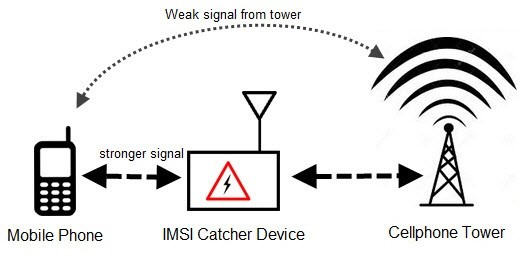
\includegraphics[width=0.5\textwidth]{images/imsi-catcher.jpg}
    \caption{Strumento per rubare IMSI}
\end{figure}\\
Questi dispositivi sono ormai semplici da reperire \textit{online} a un prezzo abbordabile per chiunque. Per rubare l'IMSI si mette in pratica un attacco di tipo \textit{Man In The Middle} (MITM), spesso utilizzato
anche per le intercettazioni da enti governativi.\\
Nelle reti di seconda generazione questo risulta molto semplice poichè come spiegato nella sezione 5.1, l'IMSI viene trasmesso in chiaro se il MS è la prima volta che si connette al registro di quella specifica
zona. Inoltre, dato che nel GSM l'autenticazione non è mutua è possibile creare una \textit{fake basestation} e collezzionare tutti gli IMSI dei dispositivi che si connettono.
Sono stati introdotti diversi identificativi temporanei come il TMSI per fare in modo che l'IMSI non debba essere inviato in ogni procedura di autenticazione, ma sono tutti facilmente raggirabili poichè cambiano con una
frequenza troppo bassa.\\
In \cite{dos-imsi} viene illustrato un metodo per ottenere gli IMSI di qualsiasi dispositivo nello standard UMTS nonostante l'autenticazione mutua. Infatti viene spiegato come basti mandare al MS una \textit{user identity request} impersonandosi 
la VLR e il MS risponderà con il proprio IMSI in chiaro.
\begin{figure}[h]
    \centering
    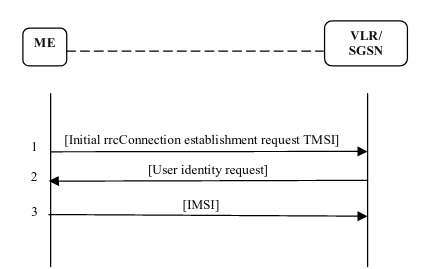
\includegraphics[width=0.5\textwidth]{images/imsi-catch-umts.png}
    \caption{IMSI \textit{catching} nelle reti UMTS\cite{dos-imsi}}
\end{figure}\\

\clearpage

\section{Attacco alle reti con dispositivi SIM-less}
In \cite{umts-dos} e \cite{gsm-dos-simless} sono descritti degli attacchi all'autenticazione degli utenti utilizzando dispositivi senza una SIM commerciale, ma bensì delle interfacce di comunicazione 
programmabili. Questo è stato fatto perchè utilizzare dei MS come dispositivi per effettuare un attacco DOS rappresenta un fattore limitante in termini di prestazioni. Infatti, 
i sistemi operativi dei MS impongono degli intervalli di tempo fra una richiesta e un'altra.\\
Entrambi gli attacchi dimostrano che è possibile causare un DOS con un numero di dispositivi senza SIM molto minore rispetto allo stato dell'arte. 
\subsection{GSM}
E' stato necessario analizzare la rispettiva \textit{air interface} del GSM per valutare quale è il numero massimo di richieste di autenticazione 
che possono essere inviate al secondo a una \textit{base station}. Questa misurazione risulta di fondamentale importanza poichè riesce anche a fornire il numero necessario 
di dispositivi per raggiungere il massimo delle \textit{transation per second} (TPS).
Nell'immagine seguente vengono illustrati i messaggi e i canali in cui viaggiano durante l'autenticazione alla rete GSM.
\begin{figure}[h]
    \centering
    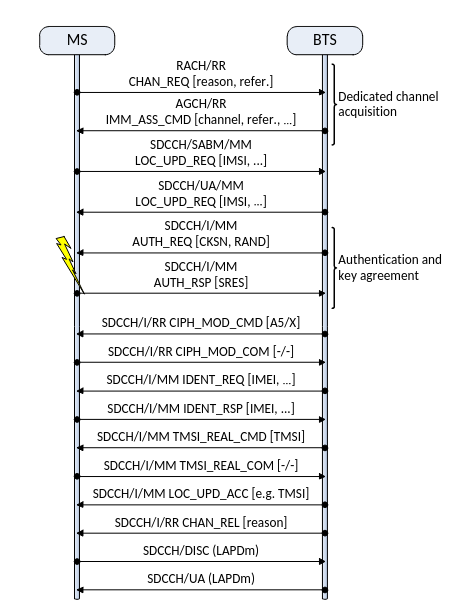
\includegraphics[width=0.5\textwidth]{images/gsm-air-channel.png}
    \caption{Messaggi scambiati durante l'autenticazione in una rete GSM\cite{gsm-dos-simless}}
\end{figure}

\clearpage

\subsection{UMTS}
L'immagine seguente rappresenta un semplice schema del dispositivo con SIM programmabile per effettuare DOS a una rete UMTS\cite{umts-dos}.
\begin{figure}[h]
    \centering
    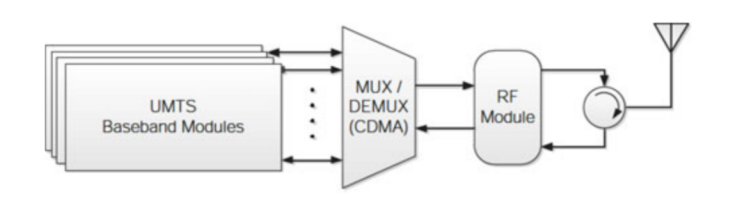
\includegraphics[width=0.5\textwidth]{images/umts-dos-device.png}
    \caption{Dispositivo per l'attacco DOS alle reti UMTS\cite{umts-dos}}
\end{figure}\\
Come è stato fatto per la rete GSM, è stato necessario analizzare l'\textit{air interface} dell'UMTS per valutare il numero di TPS.
Nell'immagine seguente vengono illustrati i messaggi e i canali in cui viaggiano durante l'autenticazione alla rete UMTS.
\begin{figure}[h]
    \centering
    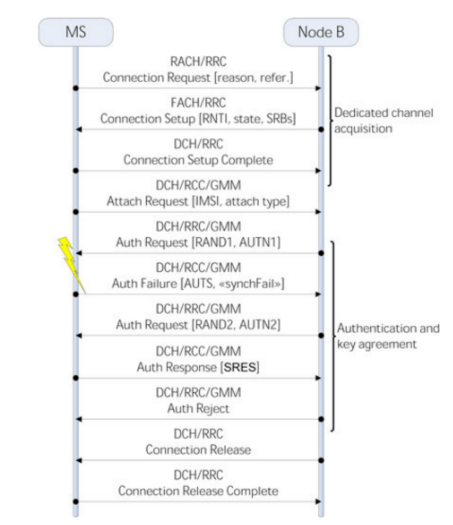
\includegraphics[width=0.5\textwidth]{images/umts-air-channel.png}
    \caption{Messaggi scambiati durante l'autenticazione in una rete UMTS\cite{umts-dos}}
\end{figure}\\
Nelle reti UMTS è stato calcolato che il limite più stringente di TPS durante la comunicazione con la \textit{base station} è dato dal canale FACH con 28 TPS.
Questo, ha portato a concludere che bastano 446 dispositivi per effettuare una notevole degradazione del sistema, molti di meno rispetto degli 11K necessari per una \textit{botnet}\cite{dos-imsi}.\\
Nello stesso articolo è spiegato come è possibile duplicare le prestazioni dell'attacco usando delle SIM valide. In questo modo infatti i vettori di autenticazione vengono generati una seconda volta se si segnala al
\textit{network} che l'AUTN calcolato non risulta corretto.
